% Options for packages loaded elsewhere
\PassOptionsToPackage{unicode}{hyperref}
\PassOptionsToPackage{hyphens}{url}
\PassOptionsToPackage{dvipsnames,svgnames,x11names}{xcolor}
%
\documentclass[
  11pt,
]{article}

\usepackage{amsmath,amssymb}
\usepackage{iftex}
\ifPDFTeX
  \usepackage[T1]{fontenc}
  \usepackage[utf8]{inputenc}
  \usepackage{textcomp} % provide euro and other symbols
\else % if luatex or xetex
  \usepackage{unicode-math}
  \defaultfontfeatures{Scale=MatchLowercase}
  \defaultfontfeatures[\rmfamily]{Ligatures=TeX,Scale=1}
\fi
\usepackage{lmodern}
\ifPDFTeX\else  
    % xetex/luatex font selection
    \setmainfont[]{Aptos}
\fi
% Use upquote if available, for straight quotes in verbatim environments
\IfFileExists{upquote.sty}{\usepackage{upquote}}{}
\IfFileExists{microtype.sty}{% use microtype if available
  \usepackage[]{microtype}
  \UseMicrotypeSet[protrusion]{basicmath} % disable protrusion for tt fonts
}{}
\makeatletter
\@ifundefined{KOMAClassName}{% if non-KOMA class
  \IfFileExists{parskip.sty}{%
    \usepackage{parskip}
  }{% else
    \setlength{\parindent}{0pt}
    \setlength{\parskip}{6pt plus 2pt minus 1pt}}
}{% if KOMA class
  \KOMAoptions{parskip=half}}
\makeatother
\usepackage{xcolor}
\setlength{\emergencystretch}{3em} % prevent overfull lines
\setcounter{secnumdepth}{-\maxdimen} % remove section numbering
% Make \paragraph and \subparagraph free-standing
\makeatletter
\ifx\paragraph\undefined\else
  \let\oldparagraph\paragraph
  \renewcommand{\paragraph}{
    \@ifstar
      \xxxParagraphStar
      \xxxParagraphNoStar
  }
  \newcommand{\xxxParagraphStar}[1]{\oldparagraph*{#1}\mbox{}}
  \newcommand{\xxxParagraphNoStar}[1]{\oldparagraph{#1}\mbox{}}
\fi
\ifx\subparagraph\undefined\else
  \let\oldsubparagraph\subparagraph
  \renewcommand{\subparagraph}{
    \@ifstar
      \xxxSubParagraphStar
      \xxxSubParagraphNoStar
  }
  \newcommand{\xxxSubParagraphStar}[1]{\oldsubparagraph*{#1}\mbox{}}
  \newcommand{\xxxSubParagraphNoStar}[1]{\oldsubparagraph{#1}\mbox{}}
\fi
\makeatother


\providecommand{\tightlist}{%
  \setlength{\itemsep}{0pt}\setlength{\parskip}{0pt}}\usepackage{longtable,booktabs,array}
\usepackage{calc} % for calculating minipage widths
% Correct order of tables after \paragraph or \subparagraph
\usepackage{etoolbox}
\makeatletter
\patchcmd\longtable{\par}{\if@noskipsec\mbox{}\fi\par}{}{}
\makeatother
% Allow footnotes in longtable head/foot
\IfFileExists{footnotehyper.sty}{\usepackage{footnotehyper}}{\usepackage{footnote}}
\makesavenoteenv{longtable}
\usepackage{graphicx}
\makeatletter
\def\maxwidth{\ifdim\Gin@nat@width>\linewidth\linewidth\else\Gin@nat@width\fi}
\def\maxheight{\ifdim\Gin@nat@height>\textheight\textheight\else\Gin@nat@height\fi}
\makeatother
% Scale images if necessary, so that they will not overflow the page
% margins by default, and it is still possible to overwrite the defaults
% using explicit options in \includegraphics[width, height, ...]{}
\setkeys{Gin}{width=\maxwidth,height=\maxheight,keepaspectratio}
% Set default figure placement to htbp
\makeatletter
\def\fps@figure{htbp}
\makeatother

\usepackage{booktabs}
\usepackage{longtable}
\usepackage{array}
\usepackage{multirow}
\usepackage{wrapfig}
\usepackage{float}
\usepackage{colortbl}
\usepackage{pdflscape}
\usepackage{tabu}
\usepackage{threeparttable}
\usepackage{threeparttablex}
\usepackage[normalem]{ulem}
\usepackage{makecell}
\usepackage{xcolor}
\usepackage{pdfpages}
\usepackage{fontspec}
\usepackage[bottom]{footmisc}
\setmainfont{Aptos}[Path="C:/Users/ginow/AppData/Roaming/TinyTeX/texmf-dist/fonts/truetype/aptos/", Extension=".ttf"]
\usepackage{fancyhdr}
\pagestyle{fancy}
\fancyhf{}
\fancyhead[C]{\makebox[\textwidth]{\hspace*{-1cm}
\includegraphics[height=1.9cm]{../Logotipo ENADEL/encabezado_izquierda.png} \hfill 
\includegraphics[height=1.5cm]{../Logotipo ENADEL/encabezado_derecha.png} \hspace*{-2cm}}}
\fancyfoot[L]{Subsecretaría del Trabajo}
\cfoot{\thepage}
\setlength{\footskip}{10pt}
\setlength{\skip\footins}{15pt}
\setlength{\headheight}{3cm}
\setlength{\headsep}{0.5cm}
\renewcommand{\footrulewidth}{0pt}
\floatplacement{figure}{H}
\floatplacement{table}{H}
\usepackage{geometry}
\geometry{ left=3cm, right=3cm, top=2.5cm, bottom=2.5cm }
\usepackage{placeins}
\usepackage{ragged2e}
\usepackage{float}
\usepackage{setspace}
\renewcommand{\familydefault}{\sfdefault}
\AtBeginDocument{\renewcommand{\baselinestretch}{1.5}\justifying}
\usepackage{xcolor}
\usepackage{pagecolor}
\makeatletter
\@ifpackageloaded{caption}{}{\usepackage{caption}}
\AtBeginDocument{%
\ifdefined\contentsname
  \renewcommand*\contentsname{Tabla de contenidos}
\else
  \newcommand\contentsname{Tabla de contenidos}
\fi
\ifdefined\listfigurename
  \renewcommand*\listfigurename{Listado de Figuras}
\else
  \newcommand\listfigurename{Listado de Figuras}
\fi
\ifdefined\listtablename
  \renewcommand*\listtablename{Listado de Tablas}
\else
  \newcommand\listtablename{Listado de Tablas}
\fi
\ifdefined\figurename
  \renewcommand*\figurename{Figura}
\else
  \newcommand\figurename{Figura}
\fi
\ifdefined\tablename
  \renewcommand*\tablename{Tabla}
\else
  \newcommand\tablename{Tabla}
\fi
}
\@ifpackageloaded{float}{}{\usepackage{float}}
\floatstyle{ruled}
\@ifundefined{c@chapter}{\newfloat{codelisting}{h}{lop}}{\newfloat{codelisting}{h}{lop}[chapter]}
\floatname{codelisting}{Listado}
\newcommand*\listoflistings{\listof{codelisting}{Listado de Listados}}
\makeatother
\makeatletter
\makeatother
\makeatletter
\@ifpackageloaded{caption}{}{\usepackage{caption}}
\@ifpackageloaded{subcaption}{}{\usepackage{subcaption}}
\makeatother

\ifLuaTeX
\usepackage[bidi=basic]{babel}
\else
\usepackage[bidi=default]{babel}
\fi
\babelprovide[main,import]{spanish}
\ifPDFTeX
\else
\babelfont{rm}[]{Aptos}
\fi
% get rid of language-specific shorthands (see #6817):
\let\LanguageShortHands\languageshorthands
\def\languageshorthands#1{}
\ifLuaTeX
  \usepackage{selnolig}  % disable illegal ligatures
\fi
\usepackage{bookmark}

\IfFileExists{xurl.sty}{\usepackage{xurl}}{} % add URL line breaks if available
\urlstyle{same} % disable monospaced font for URLs
\hypersetup{
  pdflang={es},
  colorlinks=true,
  linkcolor={blue},
  filecolor={Maroon},
  citecolor={Blue},
  urlcolor={Blue},
  pdfcreator={LaTeX via pandoc}}


\author{}
\date{}

\begin{document}

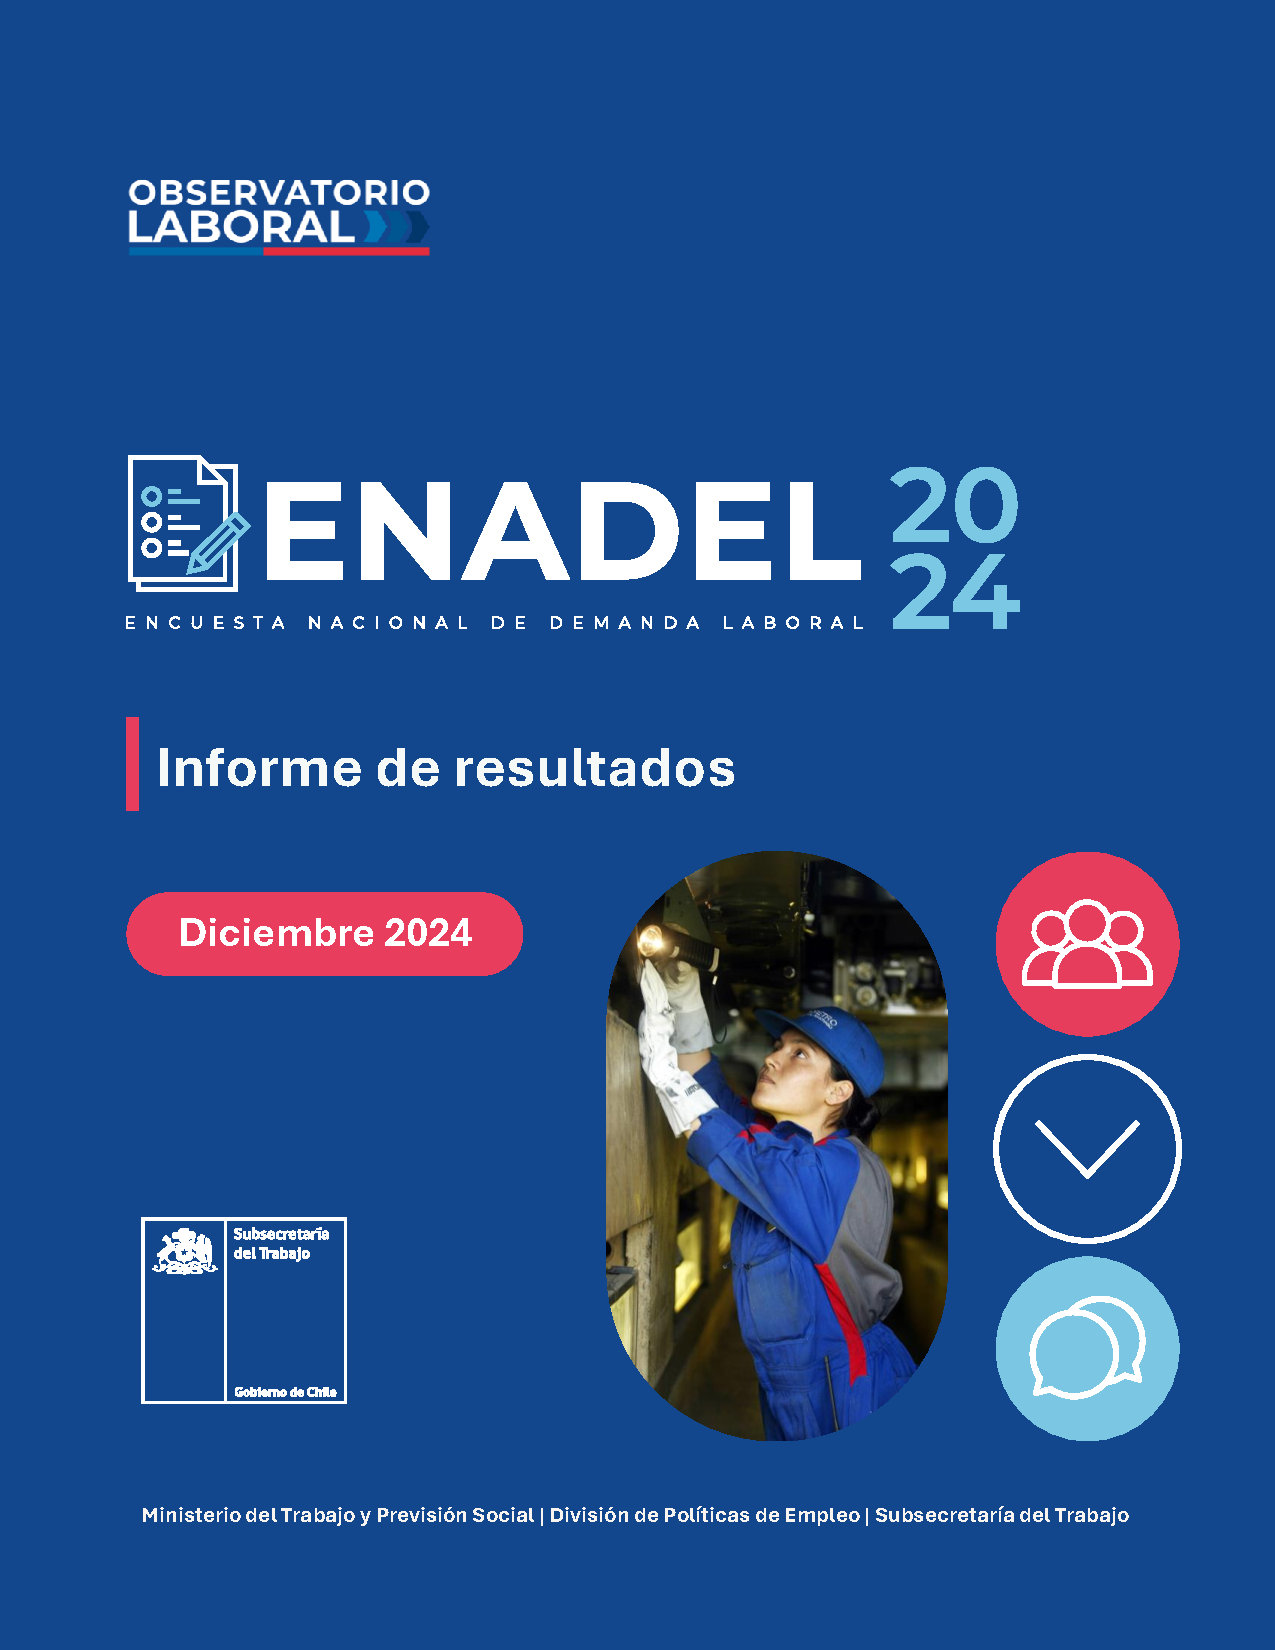
\includepdf[pages=-]{../Quarto/Portada/Portada_ENADEL 2024.pdf}


\definecolor{customblue}{HTML}{005691}

\pagecolor{customblue} 
\thispagestyle{empty} 
\color{white}

\centering


\includegraphics[width=0.5\textwidth]{../Logotipo ENADEL/Logotipo ENADEL-02.png}
\vspace{2cm}

\noindent Ministerio del Trabajo y Previsión Social

División de Políticas de Empleo\textbackslash{} Subsecretaría del
Trabajo

\justifying

El presente documento analiza los resultados de la Encuesta Nacional de
Demanda Laboral (ENADEL) 2024, que busca identificar y caracterizar el
capital humano requerido por las empresas de los distintos sectores
productivos del país, generando información sobre la demanda actual de
ocupaciones de las empresas, detectando requisitos y problemas de
contratación. A diferencia de las versiones anteriores de esta encuesta,
la actual versión abarca 15 sectores de actividad económica, ayuda a
identificar prioridades de capacitación y se añade el foco sobre el
impacto que está teniendo la incorporación de nuevas tecnologías y los
eventos climáticos extremos sobre los trabajadores.

\newpage
\nopagecolor
\color{black}
\renewcommand{\contentsname}{Índice} 
\tableofcontents

\newpage

\subsection{Capítulo I: Contexto y caracterización de
empresas}\label{capuxedtulo-i-contexto-y-caracterizaciuxf3n-de-empresas}

El primer capítulo se centra en contextualizar y caracterizar a las
empresas participantes de la Encuesta Nacional de Demanda Laboral
(ENADEL) 2024. En este apartado se busca comprender la estructura y
distribución de las empresas a nivel nacional, diferenciando por tamaño,
sector productivo y dotación de personal.

Asimismo, se examinan características relevantes de las empresas que
configuran la base del mercado laboral actual, con el fin de establecer
un panorama detallado sobre la composición y dinámica de los sectores
productivos. Este análisis otorga un marco inicial para interpretar la
demanda laboral en los siguientes capítulos, destacando patrones y
diferencias que permiten identificar regiones y sectores de mayor
demanda laboral así como los desafíos futuros asociados a la generación
de empleo en el país.

\FloatBarrier

\subsubsection{Regiones y ubicación de
sucursales}\label{regiones-y-ubicaciuxf3n-de-sucursales}

{[}1{]} ``numeric''

La muestra de ENADEL 2024 encuesta a \text{4816} empresas que suman
\text{\ensuremath{3,30937\times 10^{5}}} trabajadores (a nivel
muestral). Estas representan a \text{\ensuremath{2,45339\times 10^{5}}}
empresas y \text{\ensuremath{1,7358952\times 10^{7}}} trabajadores a
nivel nacional. La Tabla~\ref{tbl-region} muestra la distribución en las
distintas regiones del país, dónde un \text{7,3}\% de las empresas y un
\text{6,1}\% de los trabajadores se encuentran en la región
Metropolitana.

\vspace{5mm}

\FloatBarrier

\begin{table}

\caption{\label{tbl-region}Resultados de la encuesta}

\centering{

\centering
\begin{tabular}{>{\raggedright\arraybackslash}p{6cm}>{\raggedright\arraybackslash}p{3cm}>{\raggedright\arraybackslash}p{3cm}}
\toprule
Región & \% Empresas & \% Trabajadores\\
\midrule
Arica y Parinacota & 3,3\% & 1\%\\
Tarapacá & 3,9\% & 1\%\\
Antofagasta & 2,2\% & 0,8\%\\
Atacama & 5,1\% & 4\%\\
Coquimbo & 7,3\% & 9,3\%\\
\addlinespace
Valparaíso & 7,7\% & 5,2\%\\
Metropolitana & 7,3\% & 6,1\%\\
O'Higgins & 9,2\% & 7,8\%\\
Maule & 9,8\% & 7,5\%\\
Ñuble & 9,9\% & 14,3\%\\
\addlinespace
Biobío & 1,6\% & 0,2\%\\
Araucanía & 2,7\% & 4,6\%\\
Los Ríos & 14,4\% & 32\%\\
Los Lagos & 7,6\% & 4\%\\
Aysén & 3,5\% & 0,8\%\\
\addlinespace
Magallanes & 4,4\% & 1,4\%\\
\bottomrule
\multicolumn{3}{l}{\rule{0pt}{1em}Fuente: Elaboración propia utilizando datos de ENADEL 2024, datos expandidos.}\\
\end{tabular}

}

\end{table}%

\newpage

La Figura~\ref{fig-mapa-sucursal} ilustra las regiones donde las
empresas tienen sucursales, las regiones con más cantidad de sucursales
que corresponden a sedes no principales son 13110, 8739 y 8236 con un
total de 911.942961319221, 760.185838786614 y 738.767892728449
sucursales respectivamente. Por su parte, las regiones de 1907, 2081 y
2158 registran la menor presencia de sucursales regionales de las
empresas, con 387.979167200371 o menos dependencias.

\FloatBarrier

\begin{figure}[H]

\caption{\label{fig-mapa-sucursal}Sucursales por región}

\centering{

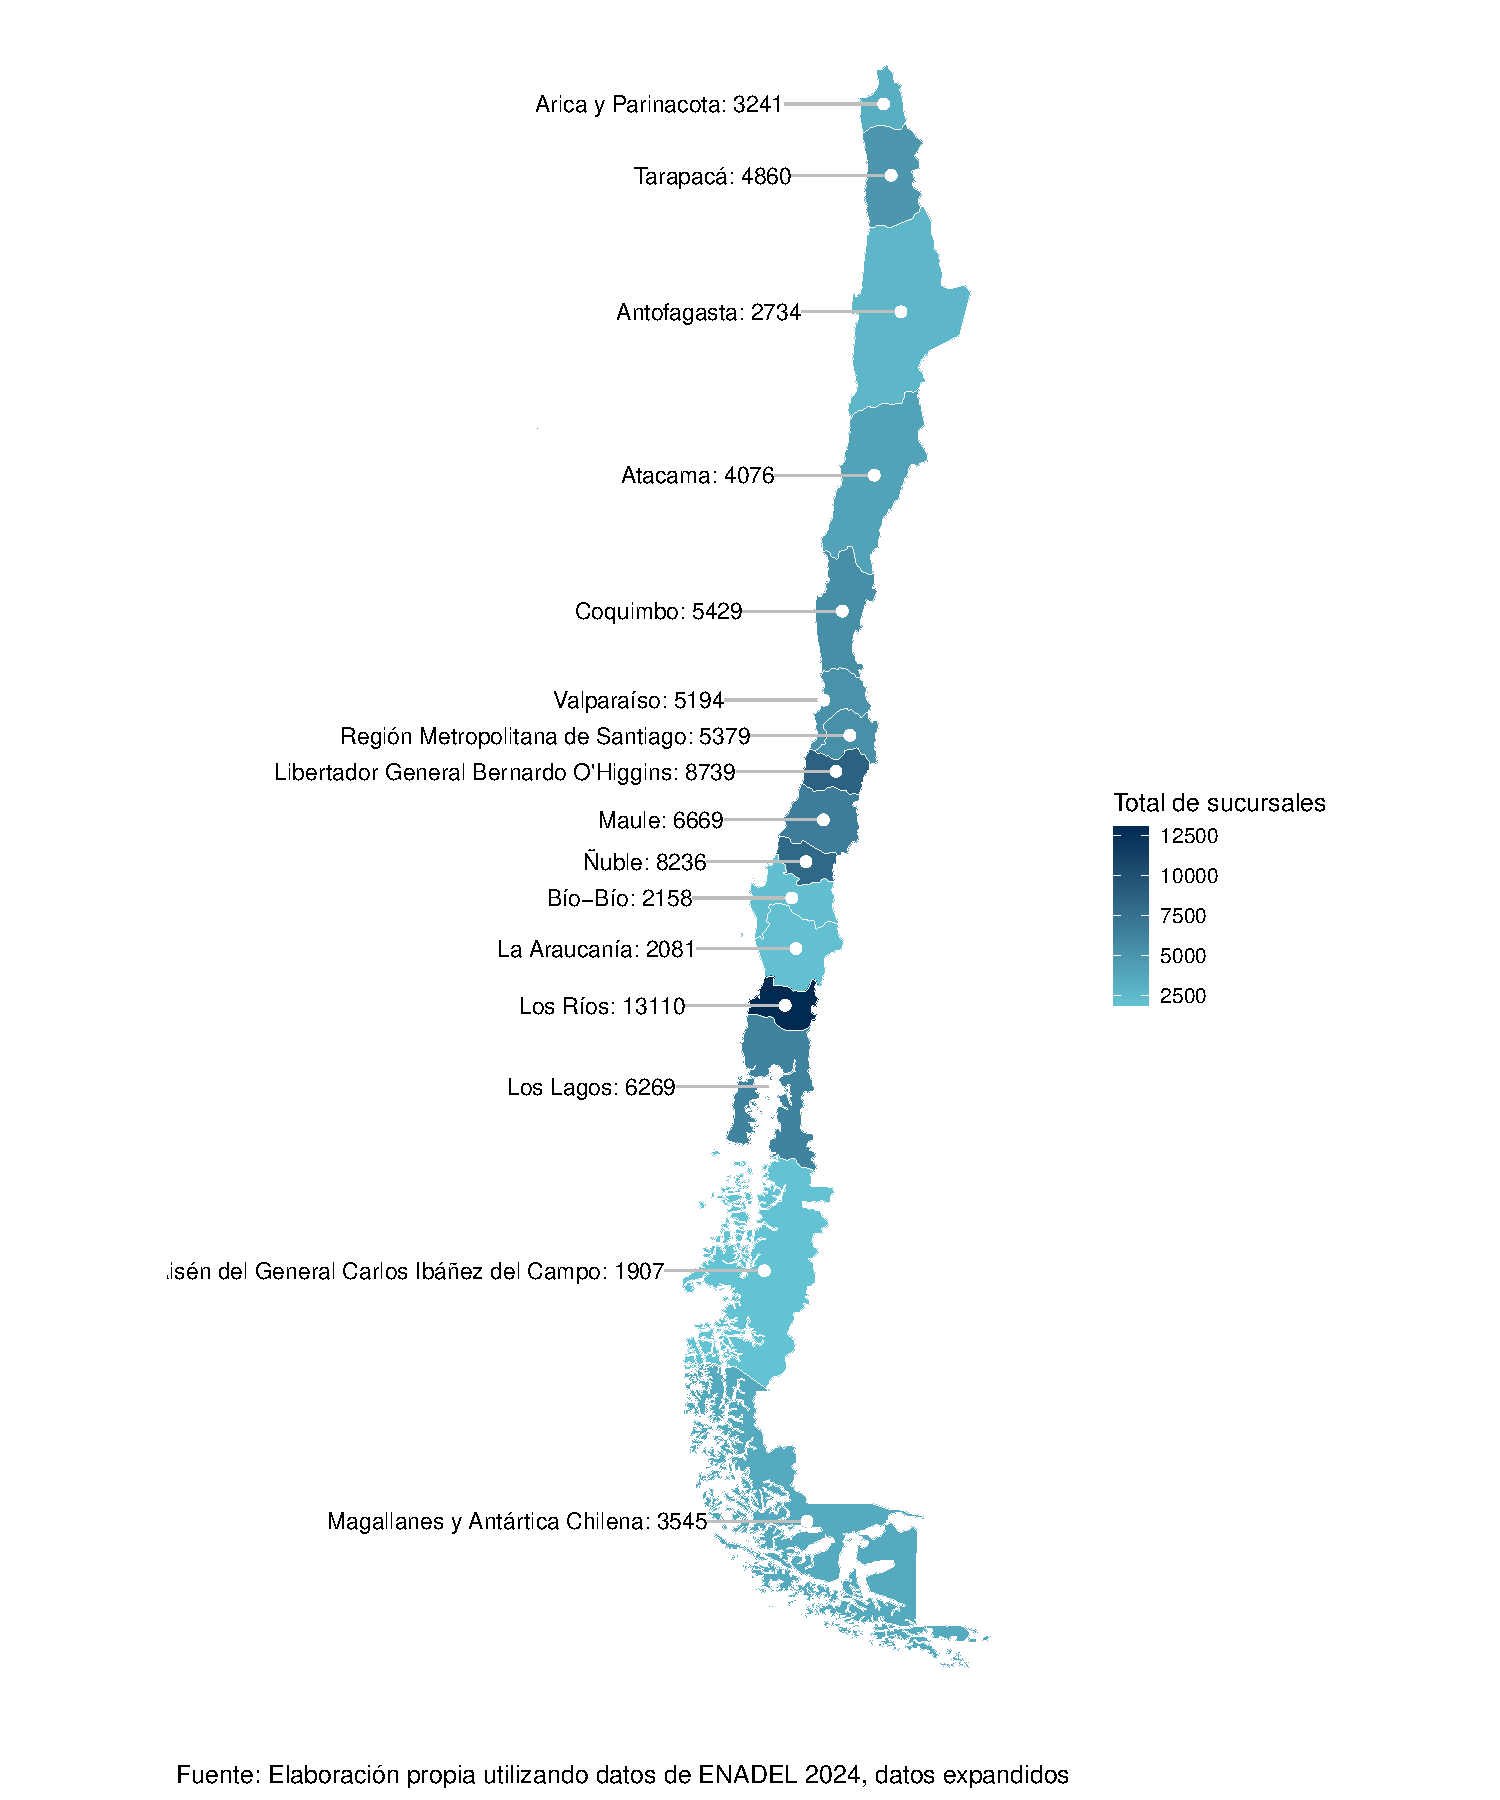
\includegraphics{reporte_2024_files/figure-pdf/fig-mapa-sucursal-1.pdf}

}

\end{figure}%

\FloatBarrier

\subsubsection{Tamaño de empresas (n° de ventas y n° de
trabajadores)}\label{tamauxf1o-de-empresas-n-de-ventas-y-n-de-trabajadores}

La Figura~\ref{fig-combined} muestra el porcentaje de empresas y
trabajadores según tamaño de empresas, utilizando la clasificación por
número de trabajadores, cómo por volumen de venta. Con respecto a la
primera clasificación, el 74,6\% de las empresas tiene menos de 50
trabajadores --acumulando un 23,8\% del total-- y casi el 50\% de los
trabajadores están en empresas grandes --que corresponden a un 6,5\% del
total. Si se analiza según tamaño de ventas, más de la mitad de las
empresas tienen un volumen de venta de entre 2.400 y 24.999 UF
(``Pequeñas'') y más de un cuarto venden entre 25.000 y 100.000 UF al
año (``Mediana''). Sin embargo, casi un tercio de los trabajadores están
en empresas grandes (más de 100.000 UF).

\FloatBarrier

\begin{figure}[H]

\caption{\label{fig-combined}Gráfico combinado de resultados}

\centering{

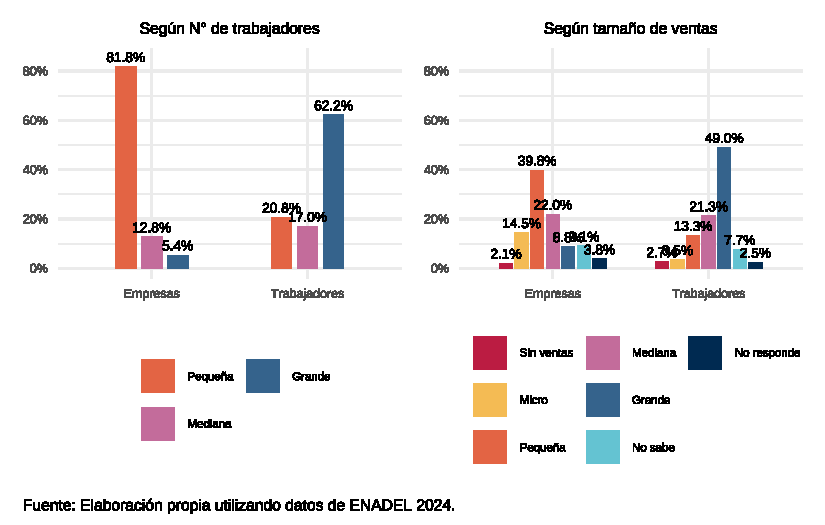
\includegraphics[width=1\textwidth,height=\textheight]{reporte_2024_files/figure-pdf/fig-combined-1.pdf}

}

\end{figure}%

\FloatBarrier

Al revisar la distribución por sector de actividad económica
Tabla~\ref{tbl-acteco} se tiene que el sector de Construcción
(\text{19}\%) , seguido por el sector Transporte y almacenamiento
(\text{14,3}\%) y el sector de Minería (\text{11,1}\%) concentran la
mayor cantidad de empresas a nivel nacional. Con respecto al volumen de
trabajadores, el sector Actividades profesionales y técnicas lidera
(\text{17,7}\%) seguido por el sector Suministro de agua y gestión de
desechos (\text{15,4}\%) y el sector de Agricultura, silvicultura y
pesca que, siendo sector intensivo en trabajo, un \text{9}\% de las
empresas acumula el \text{14,4} de trabajadores y trabajadoras.

\FloatBarrier

\begin{table}

\caption{\label{tbl-acteco}Empresas y trabajadores según sector de
actividad económica}

\centering{

\centering
\begin{tabular}{>{\raggedright\arraybackslash}p{11cm}ll}
\toprule
Actividad Económica & \% Empresas & \% Trabajadores\\
\midrule
Actividades profesionales y técnicas & 8,3\% & 17,7\%\\
Suministro de agua y gestión de  desechos & 9,9\% & 15,4\%\\
Agricultura, silvicultura y pesca & 9\% & 14,4\%\\
Construcción & 19\% & 14,2\%\\
Minería & 11,1\% & 11,4\%\\
\addlinespace
Comercio & 9,4\% & 8,6\%\\
Transporte y almacenamiento & 14,3\% & 5\%\\
Actividades inmobiliarias & 4,9\% & 3,6\%\\
Suministro de electricidad y gas & 2,3\% & 2,8\%\\
Servicios administrativos y de apoyo & 2,8\% & 2,1\%\\
\addlinespace
Alojamiento y de servicio de comida & 3,6\% & 1,8\%\\
Actividades financieras y de seguros & 3,2\% & 1,7\%\\
Industrias manufactureras & 1,1\% & 0,7\%\\
Información y comunicaciones & 1,2\% & 0,7\%\\
\bottomrule
\multicolumn{3}{l}{\rule{0pt}{1em}Fuente: Elaboración propia utilizando datos de ENADEL 2024, datos expandidos.}\\
\end{tabular}

}

\end{table}%

\FloatBarrier

\subsubsection{Estructura corporativa
(conglomerado/subcontrato)}\label{estructura-corporativa-conglomeradosubcontrato}

La Tabla~\ref{tbl-conglomerado_gremio} presenta los porcentajes de las
empresas que pertencen a conglomerados y gremios. Se aprecia que los
sectores de Comercio con el Transporte y almacenamiento y Agricultura,
silvicultura y pesca poseen los mayores niveles de empresas
conglomeradas con el 14.7\%, 11.7\% y 11.6\% de empresas
correspondientes.

Con respecto al poder asociativo de las empresas, el 15.6\% de las
empresas del sector Comercio pertenecen a un gremio empresarial. De
igual forma, el sector Alojamiento y de servicio de comida presenta un
15.6\% de empresas asociadas, mientras que el sector 15.6\% cuenta con
un Construcción de empresas pertenecientes a algún gremio empresarial.

\FloatBarrier

\begin{table}

\caption{\label{tbl-conglomerado_gremio}Empresas pertenecientes a
Conglomerados y Gremios}

\centering{

\centering
\begin{tabular}{>{\raggedright\arraybackslash}p{11cm}ll}
\toprule
Actividad Económica & \% Conglomerados & \% Gremios\\
\midrule
Comercio & 14,7\% & 15,6\%\\
Transporte y almacenamiento & 11,7\% & 10\%\\
Agricultura, silvicultura y pesca & 11,6\% & 10,1\%\\
Industrias manufactureras & 11,2\% & 11\%\\
Construcción & 10,7\% & 14,5\%\\
\addlinespace
Servicios administrativos y de apoyo & 9,5\% & 4,6\%\\
Alojamiento y de servicio de comida & 6,8\% & 15,6\%\\
Actividades inmobiliarias & 5,5\% & 3,9\%\\
Actividades profesionales y técnicas & 3,7\% & 4,2\%\\
Actividades artísticas y recreativas / Otras actividades de servicios. & 3,7\% & 1,7\%\\
\addlinespace
Actividades financieras y de seguros & 3,7\% & 1,4\%\\
Información y comunicaciones & 3,3\% & 4,5\%\\
Suministro de agua y gestión de  desechos & 2\% & 1,8\%\\
Suministro de electricidad y gas & 1,8\% & 1\%\\
\bottomrule
\multicolumn{3}{l}{\rule{0pt}{1em}Fuente: Elaboración propia utilizando datos de ENADEL 2024, datos expandidos.}\\
\end{tabular}

}

\end{table}%

\FloatBarrier

\subsection{Capítulo II: Demanda Laboral y Ocupaciones de Difícil
Cobertura}\label{capuxedtulo-ii-demanda-laboral-y-ocupaciones-de-difuxedcil-cobertura}

A continuación, se identifica y caracteriza la demanda laboral de las
empresas durante 2024. En primer lugar, se presentan las cifras
relativas a la dotación actual de personal en las empresas, seguido de
un análisis de las salidas y contrataciones realizadas para determinar
la demanda de trabajo de las organizaciones, incluyendo los principales
perfiles ocupacionales contratados, sus competencias y los requisitos
asociados.En segundo lugar, se presentan las vacantes
actuales\footnote{Número de ofertas de trabajo que se esperan abrir en
  lo que queda del año 2024.} y futuras\footnote{Número de ofertas de
  trabajo que se esperan abrir durante el año 2025.}. Para finalizar el
análisis se identifican las principales ocupaciones de difícil cobertura
presentando las dificultades más relevantes que enfrentan estas
posiciones no cubiertas.

\subsubsection{Dotación}\label{dotaciuxf3n}

En cuanto a la dotación actual de las empresas, la
Tabla~\ref{tbl-dotacion_resumen} indica que la cantidad actual de
personas empleadas asciende a un total de 17358952 a nivel nacional.
Además, se aprecia que la mayor parte de la dotación de trabajadore se
encuentra en la categoría de contrato Indefinido con un total de
11776473 trabajadores, de los cuales el 32,7\% corresponden a mujeres y
un 67,2\% a personal masculino. Si bien la distribución según sexo del
trabajador se mantiene en el resto de categorías contractuales, es la
categoría de Honorario donde hay mayor presencia de mujeres
trabajadoras, lo que da cuenta de que las mujeres se encuentran en una
condición de independencia y flexibilidad, pero al mismo tiempo de mayor
inestabilidad y ausencia de protección laboral.

\FloatBarrier

\begin{table}

\caption{\label{tbl-dotacion_resumen}Dotación actual de las empresas
segpun tipo de relación contractual}

\centering{

\centering
\begin{tabular}{>{\raggedright\arraybackslash}p{3cm}rrrll}
\toprule
Categoría & Total & Mujer & Hombre & \% Mujer & \% Hombre\\
\midrule
Indefinido & 11776472,6 & 3852312 & 7915540 & 32,7\% & 67,2\%\\
Plazo fijo & 5056494,1 & 1656658 & 3399548 & 32,8\% & 67,2\%\\
Honorario & 302954,6 & 137111 & 165803 & 45,3\% & 54,7\%\\
Dotación total & 17358952,4 & 5713742 & 11645210 & 32,9\% & 67,1\%\\
\bottomrule
\multicolumn{6}{l}{\rule{0pt}{1em}Fuente: Elaboración propia utilizando datos de ENADEL 2024, datos expandidos.}\\
\end{tabular}

}

\end{table}%

\FloatBarrier

\subsubsection{Vacantes y Salidas}\label{vacantes-y-salidas}

La Figura~\ref{fig-vacantes} presenta las vacantes actuales\footnote{Número
  de ofertas de trabajo o vacantes abiertas al 31 de mayo del 2024.} y
las vacantes futuras, que corresponden a la cantidad estimada de puestos
de trabajo que se abrirán en los próximos doce meses. Actualmente,
existen 964882 vacantes disponibles. En cuanto a las vacantes futuras,
estas se dividen en dos categorías: los puestos de trabajo previstos
para el resto del año 2024 (3235711) y las ofertas de empleo proyectadas
para el año 2025 (4620639).

\FloatBarrier

\begin{figure}[H]

\caption{\label{fig-vacantes}Gráfico Vacantes}

\centering{

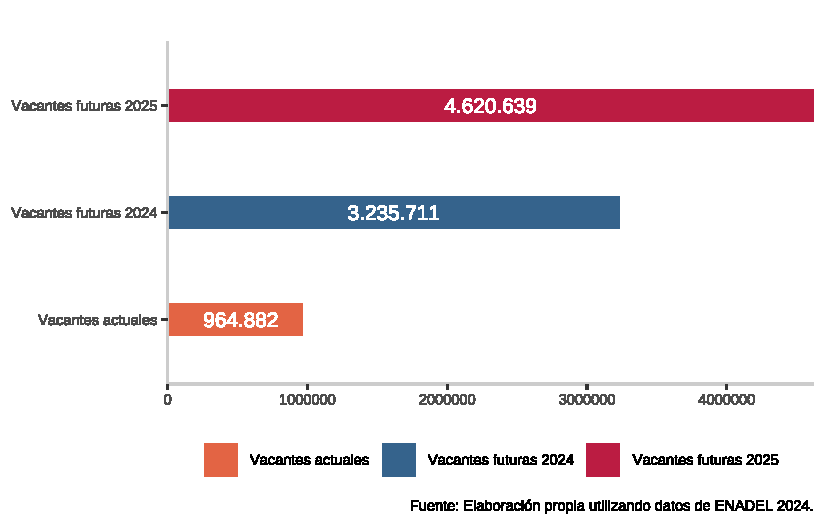
\includegraphics[width=1\textwidth,height=\textheight]{reporte_2024_files/figure-pdf/fig-vacantes-1.pdf}

}

\end{figure}%

En la Figura~\ref{fig-salidas_contrataciones} aparecen los porcentajes
correspondientes a las salidas (renuncias, despidos o ceses)\footnote{Renuncias
  y Ceses, terminaciones de empleados/as permanentes, de corto plazo o
  estacionales.} y contrataciones diferenciando por sexo de los
trabajadores. Durante los últimos 12 meses a nivel nacional hubo un
total de 1569395 renuncias, de las cuales el 34.7\% corresponde a
renuncias hechas por mujeres, mientras que el 64.5\% de estas
corresponden a renuncias hechas por hombres.

En cuanto a despidos (y ceses) \footnote{Ceses, terminaciones de
  empleados/as permanentes, de corto plazo o estacionales.}, en el
gráfico se observa que a nivel nacional existió un total de 7040137, de
los cuales el 34.8\% corresponde a casos de despidos o terminaciones de
empleos ocupados por mujeres, y un 64.4\% corresponde a despidos o ceses
cuyos puestos de trabajos eran ocupados por hombres

\FloatBarrier

\begin{figure}[H]

\caption{\label{fig-salidas_contrataciones}Gráfico salidas y
contrataciones}

\centering{

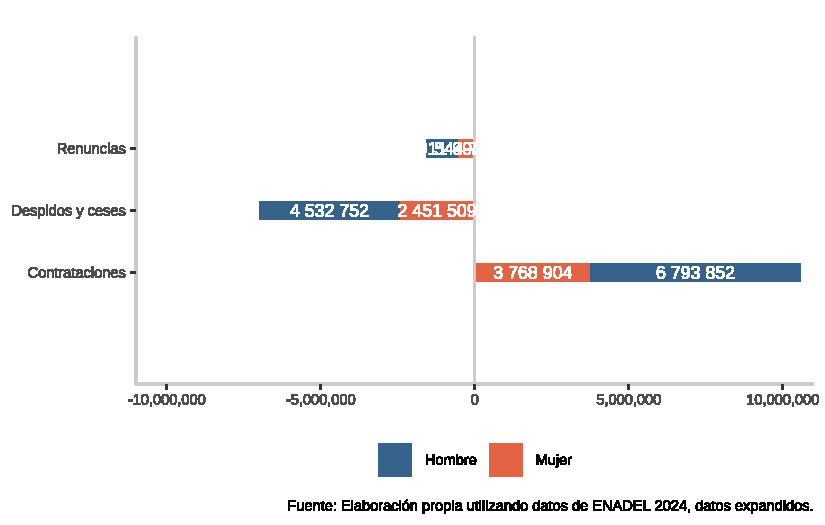
\includegraphics[width=1\textwidth,height=\textheight]{reporte_2024_files/figure-pdf/fig-salidas_contrataciones-1.pdf}

}

\end{figure}%

\subsubsection{Contrataciones últimos 12
meses}\label{contrataciones-uxfaltimos-12-meses}

la Tabla~\ref{tbl-contratados_u12} sólo muestra aquellas ocupaciones
para las cuáles el coeficiente de variación es menor a 50\%\footnote{La
  convención es considerar cómo robustas estimaciones con un cv menor al
  15\%. Dado que estas son pocas, se presentan todas las ocupaciones con
  un cv menor a 50\%.}. Las ocupaciones más contratadas en los últimos
12 meses fueron ``Auxiliares de aseo de oficinas, hoteles y otros
establecimientos'' con 222241 contrataciones, en segundo lugar con
171388 contrataciones, ``Obreros de explotaciones agrícolas'' y
``Empleados encargados del control de abastecimiento e inventario'' con
141683 contrataciones. \FloatBarrier

\begin{table}

\caption{\label{tbl-contratados_u12}Contratados últimos 12 meses, por
ocupación.}

\centering{

\centering
\begin{tabular}{r>{\raggedright\arraybackslash}p{10cm}rl}
\toprule
CIUO\_08 & Glosa & Contratados & cv\\
\midrule
9112 & Auxiliares de aseo de oficinas, hoteles y otros establecimientos & 222241 & 31,4\%\\
9211 & Obreros de explotaciones agrícolas & 171388 & 36,6\%\\
4321 & Empleados encargados del control de abastecimiento e inventario & 141683 & 34,3\%\\
5414 & Guardias de seguridad & 124867 & 48,5\%\\
3123 & Supervisores de la construcción & 86389 & 29,9\%\\
\addlinespace
3113 & Técnicos en electricidad & 85976 & 37\%\\
2142 & Ingenieros civiles, ingenieros en construcción y constructores civiles & 79051 & 34,3\%\\
9313 & Obreros de la construcción de edificios & 70138 & 36,8\%\\
4110 & Trabajadores de tareas administrativas generales & 54087 & 49,2\%\\
9412 & Ayudantes de cocina & 51284 & 32,1\%\\
\addlinespace
7112 & Albañiles & 46799 & 45\%\\
\bottomrule
\multicolumn{4}{l}{\rule{0pt}{1em}Fuente: Elaboración propia utilizando datos de ENADEL 2024, datos expandidos.}\\
\end{tabular}

}

\end{table}%

\FloatBarrier

La @tab-contratados-sector muestra la comparativa entre los sectores de
actividad económica con respecto a la cantidad de puestos de trabajos
contratados los últimos 12 meses, el sector de Agricultura, silvicultura
y pesca con 3047175 contrataciones. En segundo lugar, el sector de
Servicios administrativos y de apoyo contrató un total de 1197570
personas, seguido del sector de Construcción con un total de 498805
ocupaciones contratadas durante los últimos 12 meses. Dentro de los
sectores que menos vacantes contratados tuvieron fueron los sectores de
Actividades inmobiliarias con 27375 puestos de trabajo, el sector
Actividades financieras y de seguros con 16032vacantes contratadas y el
sector Suministro de electricidad y gas con 10017 vacantes contratadas
durante el último año.

\FloatBarrier

\begin{table}
\caption{Contratados últimos 12 meses por sector de actividad económica.}\tabularnewline

\centering
\begin{tabular}{l>{\raggedleft\arraybackslash}p{10cm}}
\toprule
Glosa & Contratados\\
\midrule
Agricultura, silvicultura y pesca & 3047175\\
Servicios administrativos y de apoyo & 1197570\\
Construcción & 498805\\
Industrias manufactureras & 449081\\
Comercio & 356693\\
\addlinespace
Transporte y almacenamiento & 253568\\
Alojamiento y de servicio de comida & 118735\\
Actividades profesionales y técnicas & 86084\\
Suministro de agua y gestión de  desechos & 44339\\
Actividades artísticas y recreativas / Otras actividades de servicios. & 37359\\
\addlinespace
Información y comunicaciones & 27481\\
Actividades inmobiliarias & 27375\\
Actividades financieras y de seguros & 16032\\
Suministro de electricidad y gas & 10017\\
\bottomrule
\multicolumn{2}{l}{\rule{0pt}{1em}Fuente: Elaboración propia utilizando datos de ENADEL 2024, datos expandidos.}\\
\end{tabular}
\end{table}

\subsubsection{Ocupaciones}\label{ocupaciones}

\subsubsection{Ocupaciones de Difícil
Cobertura}\label{ocupaciones-de-difuxedcil-cobertura}

La Tabla~\ref{tbl-cuadro8_odc} sólo muestra aquellas para las cuáles el
coeficiente de variación es menor a 40\%\footnote{La convención es
  considerar cómo robustas estimaciones con un cv menor al 15\%. Dado
  que esto no se cumple, se presentan todas las ocupaciones con un cv
  menor a 40\%.}. La ocupación más dificiles de cubrir es la de Obreros
de explotaciones agrícolas con un total de 1827 vacantes sin llenar. En
segundo lugar, la ocupación Obreros de la construcción de edificios tuvo
un total de 1438 vacantes sin llenar. La ocupación de Guardias de
seguridad tuvo un total de 1117 vacantes sin cubrir.

\begin{table}

\caption{\label{tbl-cuadro8_odc}Ocupaciones de difícil cobertura, ENADEL
2023.}

\centering{

\centering
\begin{tabular}{rlrl}
\toprule
CIUO 08 & Glosa & Vacantes & cv\\
\midrule
9211 & Obreros de explotaciones agrícolas & 1827 & 25,5\%\\
9313 & Obreros de la construcción de edificios & 1438 & 39,8\%\\
5414 & Guardias de seguridad & 1117 & 29,6\%\\
5230 & Vendedores de entradas (entretenciones y eventos deportivos) y cajeros de comercio & 1044 & 28,9\%\\
9412 & Ayudantes de cocina & 915 & 30,6\%\\
\addlinespace
5131 & Garzones de mesa & 849 & 29,1\%\\
5223 & Vendedores y asistentes de venta de tiendas, almacenes y puestos de mercado & 684 & 34,2\%\\
4110 & Trabajadores de tareas administrativas generales & 553 & 38,6\%\\
7233 & Mecánicos y reparadores de máquinas agrícolas e industriales & 513 & 36,9\%\\
3123 & Supervisores de la construcción & 512 & 37,5\%\\
\addlinespace
7212 & Soldadores y oxicortadores & 480 & 32,6\%\\
4321 & Empleados encargados del control de abastecimiento e inventario & 444 & 39,1\%\\
5245 & Bomberos de gasolineras & -3637 & -101,9\%\\
8332 & Conductores de camiones pesados y de alto tonelaje & -7785 & -108,4\%\\
8342 & Operadores de máquinas de movimiento de tierras & -8066 & -102,4\%\\
\bottomrule
\multicolumn{4}{l}{\rule{0pt}{1em}Fuente: Elaboración propia utilizando datos de ENADEL 2024, datos expandidos.}\\
\end{tabular}

}

\end{table}%

\subsubsection{Principales Dificultades}\label{principales-dificultades}

La Tabla~\ref{tbl-dificultad} muestra las principales dificultades de
contratación. La dificultad más reportada es Candidatos sin competencias
o habilidades técnicas requeridas, presente en el 24.7\% de los casos,
seguida por Falta de postulantes con un 23.7\% y Condiciones laborales
(ubicación, horario y/o jornada) no aceptadas, que representa el 10\%.

\begin{table}

\caption{\label{tbl-dificultad}Dificultades de contratación.}

\centering{

\centering
\begin{tabular}{>{\raggedright\arraybackslash}p{5cm}>{\raggedright\arraybackslash}p{3cm}}
\toprule
Primera dificultad & \% de 1ra dificultad\\
\midrule
Candidatos sin competencias o habilidades técnicas requeridas & 24,7\%\\
Falta de postulantes & 23,7\%\\
Condiciones laborales (ubicación, horario y/o jornada) no aceptadas & 10\%\\
Candidatos sin la experiencia mínima requerida & 9,5\%\\
Otra dificultad & 9\%\\
\addlinespace
Renumeración ofrecida no aceptada & 8,8\%\\
Candidatos sin habilidades blandas o socioemocionales requeridas & 7,1\%\\
Candidatos sin licencias, certificaciones o requisitos legales & 5,6\%\\
Candidatos sin nivel educacional requerido & 1,7\%\\
\bottomrule
\multicolumn{2}{l}{\rule{0pt}{1em}Fuente: Elaboración propia utilizando datos de ENADEL 2024, datos expandidos.}\\
\end{tabular}

}

\end{table}%

\subsection{Capítulo III: Capacitación y
Habilidades}\label{capuxedtulo-iii-capacitaciuxf3n-y-habilidades}

\subsubsection{Organismo Técnico Intermedio para
capacitación}\label{organismo-tuxe9cnico-intermedio-para-capacitaciuxf3n}

\subsubsection{Capacitaciones de la
empresa}\label{capacitaciones-de-la-empresa}

\subsubsection{Competencias en que se
capacita}\label{competencias-en-que-se-capacita}

\subsubsection{Fuentes de financiamiento de la
capacitación}\label{fuentes-de-financiamiento-de-la-capacitaciuxf3n}

\subsection{Capítulo IV:
Transiciones}\label{capuxedtulo-iv-transiciones}

\subsubsection{Eventos climáticos
extremos}\label{eventos-climuxe1ticos-extremos}

\subsubsection{Medidas de Cuidado del
medioambiente}\label{medidas-de-cuidado-del-medioambiente}

\subsubsection{Digitalización y
Automatización}\label{digitalizaciuxf3n-y-automatizaciuxf3n}

\paragraph{Cambios en dotación de
personal}\label{cambios-en-dotaciuxf3n-de-personal}

\paragraph{Creación de nuevos puestos de
trabajo}\label{creaciuxf3n-de-nuevos-puestos-de-trabajo}

\paragraph{Dificultad para llenar
vacantes}\label{dificultad-para-llenar-vacantes}




\end{document}
